\documentclass[tikz,border=6pt]{standalone}
\usepackage{xcolor}
\usepackage{newpxtext}
\usepackage{tikz}
\usetikzlibrary{shapes.geometric, arrows.meta, positioning, calc, fit, backgrounds}

% Color Palette matching template.tex
\definecolor{SitePrimary}{RGB}{165, 124, 117}
\definecolor{DarkCharcoal}{HTML}{2B2B2B}
\definecolor{LightTaupe}{RGB}{245, 242, 240}
\definecolor{SubtleGray}{HTML}{F4F4F4}
\definecolor{BoxBorder}{HTML}{D0C9C5}
\definecolor{AccentGreen}{HTML}{2E7D32}
\definecolor{AccentBlue}{HTML}{1565C0}

\begin{document}
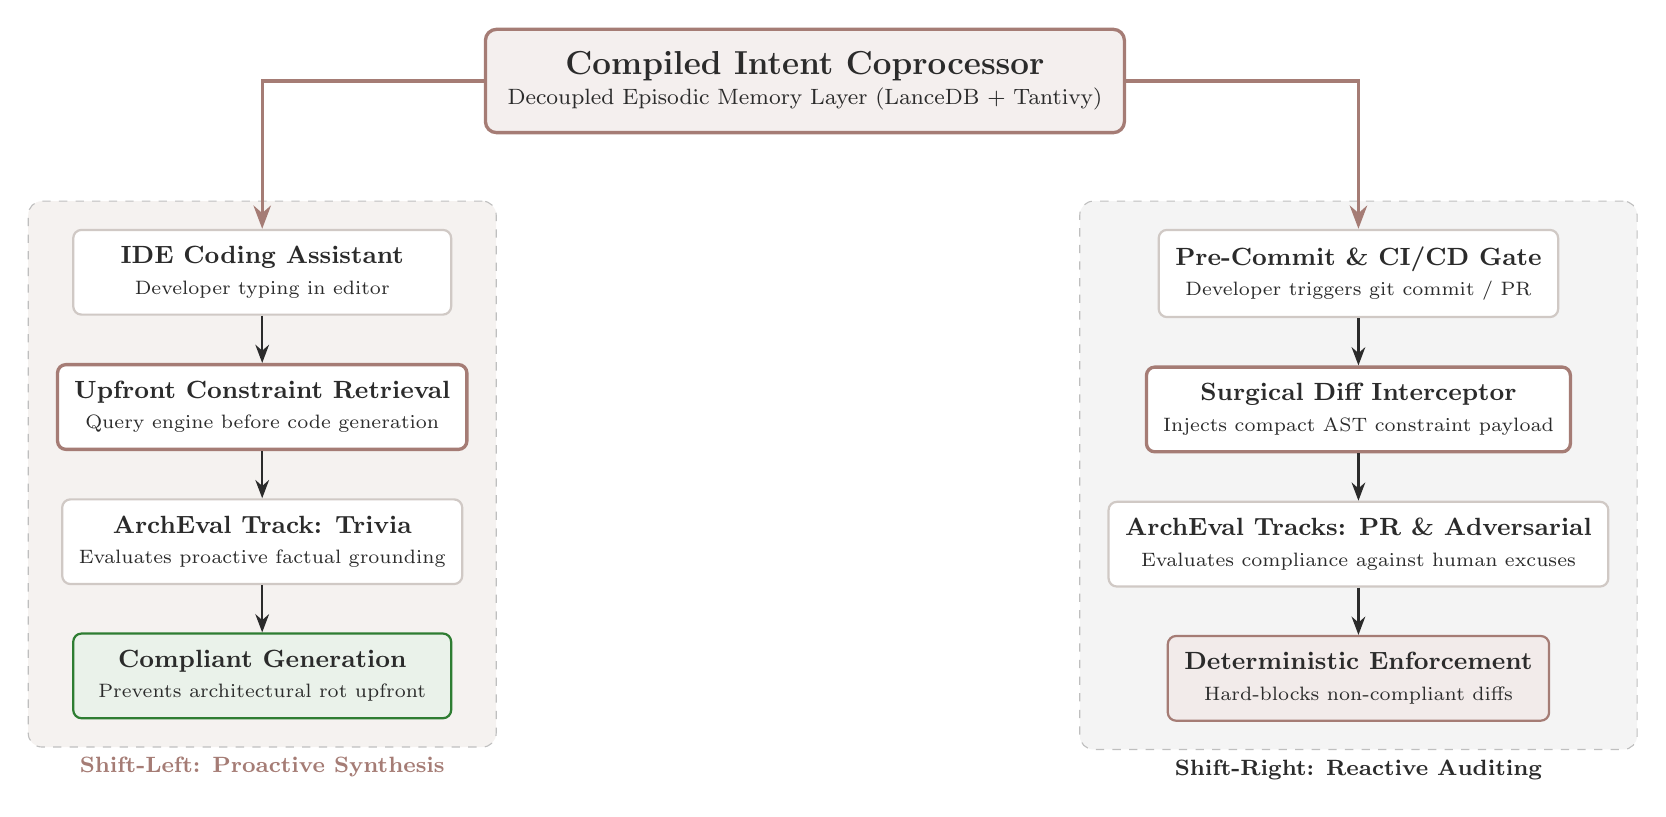
\begin{tikzpicture}[
    font=\small\color{DarkCharcoal},
    >=Stealth,
    node distance=1.4cm and 1.8cm,
    centralblock/.style={
        rectangle,
        draw=SitePrimary,
        fill=SitePrimary!12!white,
        rounded corners=4pt,
        very thick,
        align=center,
        inner sep=8pt,
        minimum height=1.2cm,
        minimum width=5.5cm
    },
    phaseblock/.style={
        rectangle,
        draw=BoxBorder,
        fill=white,
        rounded corners=3pt,
        thick,
        align=center,
        inner sep=6pt,
        minimum height=1.0cm,
        minimum width=4.8cm
    },
    highlightblock/.style={
        rectangle,
        draw=SitePrimary,
        fill=white,
        rounded corners=3pt,
        very thick,
        align=center,
        inner sep=6pt,
        minimum height=1.0cm,
        minimum width=4.8cm
    },
    subgraph/.style={
        draw=DarkCharcoal!30,
        fill=LightTaupe,
        rounded corners=5pt,
        dashed,
        inner sep=10pt
    },
    line/.style={
        ->,
        thick,
        color=DarkCharcoal
    },
    primaryline/.style={
        ->,
        very thick,
        color=SitePrimary
    }
]

    % --- Central Anchor: Compiled Intent Coprocessor ---
    \node[centralblock] (core) {\textbf{\large Compiled Intent Coprocessor}\\{\footnotesize Decoupled Episodic Memory Layer (LanceDB + Tantivy)}};

    % --- Left Column: Proactive Synthesis (Shift-Left) ---
    \node[phaseblock, below left=1.2cm and 0.4cm of core] (ide) {\textbf{IDE Coding Assistant}\\{\scriptsize Developer typing in editor}};
    \node[highlightblock, below=0.6cm of ide] (query) {\textbf{Upfront Constraint Retrieval}\\{\scriptsize Query engine before code generation}};
    \node[phaseblock, below=0.6cm of query] (trivia) {\textbf{ArchEval Track: Trivia}\\{\scriptsize Evaluates proactive factual grounding}};
    \node[phaseblock, fill=AccentGreen!10!white, draw=AccentGreen, below=0.6cm of trivia] (proactive_res) {\textbf{Compliant Generation}\\{\scriptsize Prevents architectural rot upfront}};

    % --- Right Column: Reactive Auditing (Shift-Right) ---
    \node[phaseblock, below right=1.2cm and 0.4cm of core] (commit) {\textbf{Pre-Commit \& CI/CD Gate}\\{\scriptsize Developer triggers git commit / PR}};
    \node[highlightblock, below=0.6cm of commit] (audit) {\textbf{Surgical Diff Interceptor}\\{\scriptsize Injects compact AST constraint payload}};
    \node[phaseblock, below=0.6cm of audit] (eval) {\textbf{ArchEval Tracks: PR \& Adversarial}\\{\scriptsize Evaluates compliance against human excuses}};
    \node[phaseblock, fill=SitePrimary!15!white, draw=SitePrimary, below=0.6cm of eval] (reactive_res) {\textbf{Deterministic Enforcement}\\{\scriptsize Hard-blocks non-compliant diffs}};

    % --- Subgraph Enclosures ---
    \begin{scope}[on background layer]
        \node[subgraph, fit=(ide) (query) (trivia) (proactive_res), label={[font=\footnotesize\bfseries\color{SitePrimary}, anchor=north]south:Shift-Left: Proactive Synthesis}] (leftbox) {};
        \node[subgraph, fit=(commit) (audit) (eval) (reactive_res), fill=SubtleGray, label={[font=\footnotesize\bfseries\color{DarkCharcoal}, anchor=north]south:Shift-Right: Reactive Auditing}] (rightbox) {};
    \end{scope}

    % --- Connections ---
    \draw[primaryline] (core.west) -| (ide.north);
    \draw[primaryline] (core.east) -| (commit.north);

    \draw[line] (ide) -- (query);
    \draw[line] (query) -- (trivia);
    \draw[line] (trivia) -- (proactive_res);

    \draw[line] (commit) -- (audit);
    \draw[line] (audit) -- (eval);
    \draw[line] (eval) -- (reactive_res);

\end{tikzpicture}
\end{document}
